\chapter{Access Control}

\section{Introduction}

The main tasks of the security system will be to ensure proper access
for the users and protect the structure and the content of any APIIS
databases from unauthorized actions. 

APIIS needs guarantees that the persons connecting to the system
are really the ones they claim to be and also has to control the actions
each person is trying to perform. 


\section{Requirements for the access control system }

The requirements for the APIIS security system have two components: 

\begin{itemize}
\item Access rights, 
\item Side conditions. 
\end{itemize}

\subsection{Access rights }

In our case we can define two groups of access rights: 

\begin{itemize}
\item access rights for the programs, 
\item access rights for the database and the content of the database. 
\end{itemize}
We are looking for a means to restrict the access of individual users
to specific subsets of the available data in the same data model.
That means we have to define the following objects, targets and actions
for our databases: 

\begin{description}
\item [Objects~and~targets:]We define the following access rights for
database: 
\end{description}
\begin{itemize}
\item user validation, 
\item access rights restricted for each table, 
\item access rights restricted for each column in database,
\item access rights to be specified on row content.
\end{itemize}
\begin{description}
\item [Actions:]This access rights have to be specified for operation on
data as follows:
\end{description}
\begin{itemize}
\item select - possibility to read record,
\item insert - possibility to add new record,
\item update - possibility to change existing record,
\item delete - possibility to delete existing record.
\end{itemize}
\begin{description}
\item [Programs~to~move~up:]Definition of rules and access rights for
the file system is the next important thing. We have to define them
because not each user will have access to all file (for instance:
model file, scripts file). User can only execute or edit files which
are defined in his individual access rights (for instance if user
login to the system he has only list of jobs which are granted to
him by administrator). 
\end{description}

\subsection{Side conditions }

Security system should be an independent access control system and
cooperate with various database systems. We have to consider two main
ways of independence: independence from operating system and independence
from the type of database. 

\begin{description}
\item [Independence~from~operating~system:]We have many various operating
systems. Our solution should be universal and work with every operating
system: Linux, Windows, ... . 
\item [Independence~from~type~of~database:]There are a few database
environment. We have to create system that will collaborate with different
database engines like PostgreSQL, Oracle, MySQL. 
\end{description}

\section{Implementation of access control system }

\subsection{System architecture}
There are three logical machines in an APIIS database setup (Figure \ref{fig:schema}): 
\begin{itemize}
\item client machine - the machine at which a users types 
\item APIIS server - the machine that all users connect to
\item Database server - the machine that runs the backend database
\end{itemize} 
Clearly, all three logical machines can reside on one or more physical computers.\\
The APIIS Server takes care of the authentication of the users, 
connections to the database server and presenting data back to the users on the operating
system level. Thus, to execute a program each user must have an account in operating system 
on the server, that means each individual user must have a login/password on the APIIS Server.
This is the standard route to get access to the data for both reading and modifications. 
Following this route, the user has to log in via ssh protocol on the APIIS server. 
In case of successful authentication on the operating system level, graphical interface is 
started on the server side by the login command, allowing the user to access only his 
set of programs.\\ 

All software resides on the APIIS Server and is used by all users. This means that programs are executed on the server and all users use the same libraries and modules. This also means that there is only one model file for everyone, located on this server. In such environment all APIIS resources have to be placed in some secure space on the server and have to be protected against modifications by not allowed persons.

The general schema how the system is implemented is shown on Figure \ref{fig:generalschema}.
\begin{figure}[h]
\begin{center}
   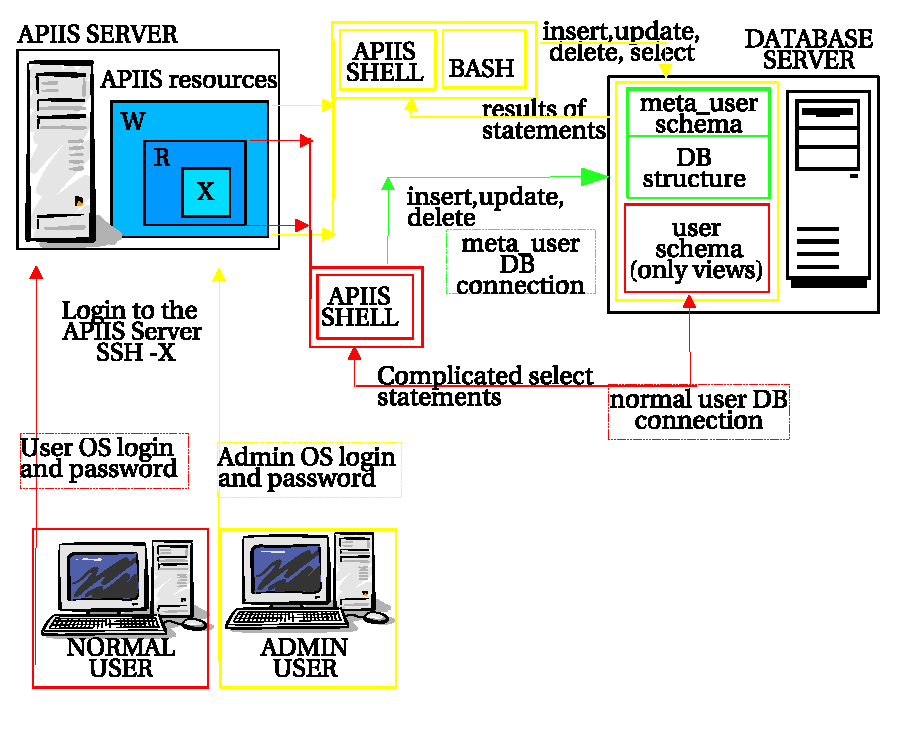
\includegraphics[scale=1]{./access-control/generalschema.eps}
   \caption{General schema for the access control system}
   \label{fig:generalschema}
\end{center}
\end{figure}

\subsection{Definitions of the user \label{userd}}
Only registered users can work in the system. Each user has to be registered on the three levels: 
\begin{itemize}
\item operating system level,
\item database level, 
\item apiis system level.
\end{itemize} 
\subsubsection{Operating system level}
User has to have an account (login and password) in the operating system. For example to create a standard Linux user, you have to run this command:
\begin{verbatim}
adduser [login] -g [login]
\end{verbatim} 
When user's account is created then the APIIS\_HOME path have to be defined in .bashrc or .profile file. Path have to be redirected to the apiis administrator space - place where the software is keept (\ref{filesysard}).
\begin{verbatim}
Example:
export APIIS_HOME=/home/apiis/devel/apiis
\end{verbatim} 
\subsubsection{Database level}
Apiis system is based on PostgreSQL database and to work with it user needs database account. Database account for the user has to be created with the password and it name has to be the same like a operating system user name. Standard user should not have access rights to create new database and create new user. This database account is needed for log-in to the system and to permit user to executes some complicated SQL SELECTs. These SQL SELECTs statement are executed on the views which are created separatly for each user. The views are created in user schema on basis user access rights. User can only execut selects and all another access rights are revoked from him. Even if he log-in to the database via psql command he can do nothing.\\
There is only one model file for everyone located on the APIIS server and there is also one meta\_user written in this file that has access rights to the database without any restrictions. All database is placed in his schema (to do this, you have to remove PUBLIC schema and creates your database in the meta\_user schema). This meta\_user is responsible for all modifications in the database and nobody else can do this. When the user executes a query, the connection to the database is established from the meta\_user. Real user name is used to check user access rights. Then the meta\_user run all processes if the user has authorization for this action. Real user name is also sent as a normal data for the meta fields (last\_change\_user).
The results from the query are shown via the APIIS interface. The
schema is shown on Figure 

\subsubsection{Apiis system level}
To work with apiis, user needs also special account inside this system. Folowing data about user are collected in the database:
\begin{itemize}
\item login,
\item password, 
\item first name and last name,
\item country,
\item language
\end{itemize}   
On basis this account all access right are checked.

\subsection{Access control for the applications and the interface\label{acftaati}} 
\subsubsection{Definitions of the access rights \label{filesysard}} 
 
Definition of the access rights for the applications (files) is based on the usege some secure space on the server. This secure space is received by creating a special administrator account (OS account). Administrator is the owner of the files and he has full rights to reading, writing and executing. Access to these files for another users is handled by the special groups. Each file has defined group to which belong and special rights for this group (reading, writing and executing). In our case all files are defined in the apiis group (this group is created with apiis user account). This apiis group can be ascribed to each operating system user and with this group user has rights only to the reading and executing files. Other users which are not in the apiis group can only read the files. There are also some exceptions when some of the files have to be fully restricted for the users (some administrator modules). This can be done by removing all rights from the apiis group and from the other users. In this case only administrator has access to these files.
\\
Some of the applications or scripts can change database structure or content and not each user may have access to them. We have to be sure that user runs only these applications which are allowed for him. This means that each user has to have defined own access rights for the applications. The definition of the access rights is based on the roles - roles based system. In this type of system each role is a definition of the group of the access rights and can be assigned to many users. In the roles, access rights are defined via policies. In our case each policy defines access to one application/file or the action for the interface.
All access rights for the application are stored in database tables. To store this data we use following tables:
\begin{itemize}
\item users table - this table stores information about the users,

\begin{table}[h]
\begin{center}\begin{tabular}{|c|c|c|c|c|c|}
\hline 
user\_id&login&password&name&country&language\tabularnewline
\hline
\hline
1&kloss&***&Hans Kloss&Germany&German\tabularnewline
\hline 
2&user&***&User User&Poland&Polish\tabularnewline
\hline 
\end{tabular}\end{center}
\caption{Users table}\label{Usertable1}
\end{table}

\item roles table - this table stores information about the roles,

\begin{table}[h]
\begin{center}\begin{tabular}{|c|c|c|}
\hline 
role\_id&role\_name&role\_type\tabularnewline
\hline 
1&sys\_admin\_role&DB\tabularnewline
\hline 
2&public\_role&OS\tabularnewline
\hline 
3&db\_admin\_role&DB\tabularnewline
\hline 
\end{tabular}\end{center}
\caption{Roles table}\label{rolestable1}
\end{table}

\item policies for the applications - this table stores information about file names.


\begin{center}%
\begin{table}[h]
\begin{center}\begin{tabular}{|c|c|c|}
\hline 
app\_policy\_id&
action name&
action class
\tabularnewline
\hline
\hline 
1&
runall\_ar.pl&
program
\tabularnewline
\hline 
2&
enter data&
www
\tabularnewline
\hline 
3&
add new user&
action
\tabularnewline
\hline 
4&
number of animals in year 2004&
report
\tabularnewline
\hline
\end{tabular}\end{center}
\caption{Policies for the applicatios}\label {policiestable1}
\end{table}
\end{center}
\end{itemize}

The realtions beetwen these tables are keept in separate two tables.

\subsubsection{Checking of the access rights - loging to the system}
There are two ways to work with the APIIS system:
\begin{itemize}
\item directly on the APIIS server (via ssh),
\item APIIS web page (via web browser). 
\end{itemize}

If user wants to work directly on the APIIS server first has to connect via ssh to the server (OS login and password). After log-in to the server, special apiis shell is activated for the user. On the beginning this shell contains only some initial forms and informations. There is also log-in options in this shell which user has to use to connect to the database. User has to specify here his database login, password and database name. If data are consistent then the meta\_user has to check user access rights for the applications. The meta\_user log-in to the database ( the internal system connection) and checks in the tables which application user can execute. List of the applications is returned in result. This list is loaded in to the apiis shell. Finally user has only these applications and forms to which he is in the right.
After log-in via ssh to the APIIS server user can also execute some scripts (from the command line) if he is allowed to this. Procedure of checking access right for current applications is the same like during log-in via apiis shell. Difference here is that the meta\_user checks access right only for this application.  

Second variant to work with the APIIS is web browser. Here instead of connection to the server user has to specify correct address to the APIIS internet page. Login procedure is exacly the same like for the apiis shell. The
schema is shown on Figure \ref{fig:serverloging}.
\begin{figure}[h]
\begin{center}
   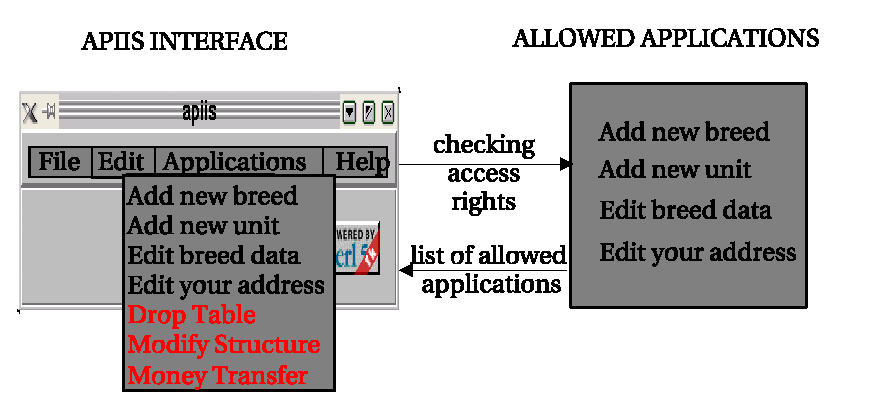
\includegraphics[scale=1]{./access-control/serverloging.eps}
   \caption{Loging to the APIIS system}
   \label{fig:serverloging}
\end{center}
\end{figure}

\subsection{Access control for the database and the content of the database}
We define two different methods for checking access rights on the database level. The choice of which
depends on type of the SQL Statement which is executed.
One applies only to \emph{insert/update/delete}
statements while another is used for \emph{select} statements. The type of the SQL
Statement is recognized on the beginning and then the relevant method
is launched.


\subsubsection{Method for the insert, update and delete statements \label{pseudosql}}

This route is especially for insert, update and delete statements (pseudosql select statements are also allowed).
This method can be describe by following steps: 
\begin{enumerate}
\item all actions go through the meta-layer,
\item each DML call is sent through the DBI in the meta-layer and the action
is checked for the user,
\item the arguments in the action (table/columns) are matched with the access
rights defined for this user,
\item if the user doesn't have the required access rights for this table/columns
set the action is aborted, 
\item if the user have access rights for this operation, the DML call is
modified via adding arguments to the WHERE clause. These arguments
are classes of records on which user can execute this operation.
\end{enumerate}

\paragraph {Definition of the access rights:}
	
Definition of the access rights is also based on roles (the roles based system) like was defined for the applications (\ref{filesysard}). 
Here also all access rights are grouped in roles and each user who wants to work with the database,
has ascribed one or a few roles. Role defines access rights to the group of tables,
columns, records. Each role consists of one or more policies. Each
policy consists of action (INSERT/UPDATE/DELETE), table name, column
names for this table and owner (class of records).

All information about database access rights are stored in the database. Here we use also two the same table which was defined for the applications (users - Table \ref{Usertable1} and roles - Table \ref{rolestable1} ). Third table is different and it store information about policies for the database (Table \ref{dbpoliciestable})
On the basis of these three tables individual view for each user with
all his access rights is created.The name of this view is 
derived from user name. This view is schown in Table \ref{userview}

\begin{center}%
\begin{table}[h]
\begin{center}\begin{tabular}{|c|c|c|c|c|}
\hline 
policy\_id&
tablename&
columnnames&
owner(class)&
action\tabularnewline
\hline
\hline 
1&
breeds&
orgin|dailygain|conditions&
PL&
INSERT\tabularnewline
\hline 
2&
publications&
title|author|language&
DE&
SELECT\tabularnewline
\hline 
3&
animal&
db\_breed|birth\_dt|db\_sex|name&
PL&
UPDATE\tabularnewline
\hline 
4&
animal&
&
PL&
DELETE\tabularnewline
\hline
5&
animal&
db\_animal|birth\_dt&
BG&
UPDATE\tabularnewline
\hline
\end{tabular}\end{center}
\caption{Policies table}\label {dbpoliciestable}
\end{table}
\end{center}

\begin{center}%
\begin{table}[h]
\begin{center}\begin{tabular}{|c|c|c|c|}
\hline 
tablename&
columnames&
class&
action\tabularnewline
\hline
\hline 
breeds&
origin|dailygain|conditions&
PL&
INSERT\tabularnewline
\hline 
publications&
title|author|language&
DE&
SELECT\tabularnewline
\hline 
animal&
db\_breed|birth\_dt|db\_sex|name&
PL&
UPDATE\tabularnewline
\hline 
animal&
&
PL&
DELETE\tabularnewline
\hline
animal&
db\_animal|birth\_dt&
BG&
UPDATE\tabularnewline
\hline
\end{tabular}\end{center}
\caption{User access rights view}\label{userview}
\end{table}
\end{center}

\paragraph{Checking of the access rights:}

The procedure of checking access rights is executed separately for each SQL statement. Each SQL statement (from LO, forms or another programs), excluding normal SELECT, is parsed and results are put into the special structure. All information about SQL statement needed for the checking of access rights is taken from this structure.

This process can be defined by the following steps: 

\begin{enumerate}
\item Action name and table name are taken from the structure.


\begin{center}\textbf{\emph{UPDATE}} \emph{}\textbf{\emph{animal}}
\emph{SET name='cow', birth\_dt='01-09-1993' WHERE db\_sex=1 }\end{center}

\begin{center}\emph{(exemplary user statement )}\end{center}

\item ''SELECT'' statement is executed on the access rights view belong to this
user. In the WHERE clause the arguments which were returned in step 1 -
action name, table name are used.
\begin{center}\emph{SELECT columnnames,class FROM v\_ar\_user WHERE
action='}\textbf{\emph{UPDATE}}\emph{' and table='}\textbf{\emph{animal}}\emph{'}\end{center}
This statement returns column names and classes of records from table
''animal'' on which this user can execute ''UPDATE'' statement.
If we look at the 'Table \ref{userview}', then we have in a result: 	

\begin{table}[h]
\begin{center}\begin{tabular}{|c|c|}
\hline 
columnnames&
class\tabularnewline
\hline
\hline 
db\_breed|birth\_dt|db\_sex|name&
PL\tabularnewline
\hline
db\_animal|birth\_dt&
BG\tabularnewline
\hline
\end{tabular}\end{center}
\caption{Allowed columns}\label{allowcolumns}
\end{table}

\item Access rights are checked; column names from user statement are matched
with allowed column names which were returned in step 2. 


Results of checking access rights can be either TRUE or FALSE: 

\begin{itemize}
\item FALSE: user statement contains a column which is not listed in the output from
step 2 i.e for this table user has no rights,
\item TRUE: all columns in the user statement have been founded in the access rights selected in step 2,
Additional extension for the WHERE clause is returned. 


This WHERE clause extension defines the range of records on which
user can execute this statement. This extension is a list of classes where
class defines the owner of the record. In EFABIS it is a shortcut that come from the country name and
each record in database have this class field.
List of classes is created during the checking access rights process. When user have access rights to the column,
class for this column is taken from the results returned in step 2 and then store in some temporary list. 
Class is added to the final list only if all columns from SQL statement have defined
access rights in this class. At the end final list of classes is added to the SQL statement.

In our case algorithm returns following class: \textbf{'PL' }

(in class 'BG' we have only access rights for the column 'birth\_dt').

\end{itemize}
\item Base SQL Statement is changed (only in case 'TRUE') by adding an
extension to the WHERE clause. Our SQL statement looks like:


\medskip{}
\begin{center}\emph{UPDATE} \emph{animal SET name='cow',
birth\_dt='01-09-1993' WHERE} \emph{(db\_sex=1} \textbf{\emph{)}} 
\textbf{\emph{and ( class='PL' )}}\end{center}
\medskip{}

\item SQL Statement is sent to execution.
\end{enumerate}
The symbolic schema is shown on Figure \ref{fig:modifingdata}.
\begin{figure}[h]
\begin{center}
   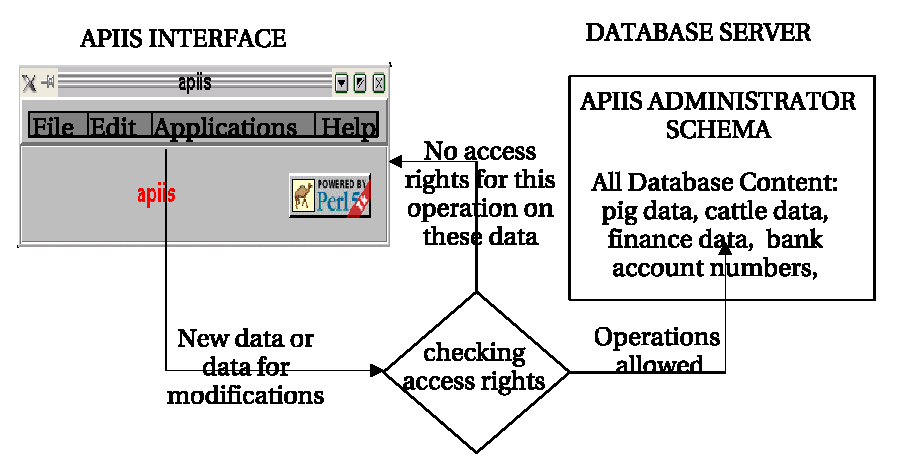
\includegraphics[scale=1]{./access-control/modifingdata.eps}
   \caption{Modifing the database content}
   \label{fig:modifingdata}
\end{center}
\end{figure}

\subsubsection{Method for the public select statements}

Access rights for the public statements (selects) follow a different route from the method
which is described in previous section \label{sec:pseudosql}. This route is different, because the parsing of a complex select statement is too complicated.
All select statements are executed directly on the user views. User can access only these views which are created in his schema. Each view contains only those rows and columns that the user is allowed to access on the basis of his access rights. For the view system each user has to have database account. This method can be describe by following steps:
\begin{enumerate}
\item user schema is created (schema is created only one time, after first log-in to the system),
\item views are created in the user schema; views are created on basis user access rights    
(views haven't to be created after each log-in but in this case we have to have some warning system or some flags. If there are some changes in access rights or original tables, flag should be changed
and then when user log-in view is recreated). 

\item each \emph{select} statement is executed directly on the database. Now the default namespace is the user own schema and the select statement will be executed on the views instead of the original tables.
\end{enumerate}


\paragraph{Definition of the access rights:}
All access rights to create views (to execute \emph{select} statements)
are defined in the same user access view like for \emph{update,
insert} and \emph{delete}.

\begin{center}%
\begin{table}[h]
\begin{center}\begin{tabular}{|c|c|c|c|}
\hline 
tablename&
columnames&
class&
action\tabularnewline
\hline
\hline 
breeds&
origin|dailygain|conditions&
PL&
INSERT\tabularnewline
\hline 
publications&
title|author|language&
DE&
SELECT\tabularnewline
\hline 
animal&
db\_breed|db\_sex|name&
PL&
UPDATE\tabularnewline
\hline 
animal&
&
PL&
DELETE\tabularnewline
\hline
animal&
db\_animal|birth\_dt&
BG&
UPDATE\tabularnewline
\hline
publications&
title|description|format|language|location&
PL&
SELECT\tabularnewline
\hline
publications&
title|author|language|size|date&
BG&
SELECT\tabularnewline
\hline
animal&
db\_animal|db\_breed|db\_sex\_db\_name&
PL&
SELECT\tabularnewline
\hline
\end{tabular}\end{center}
\caption{User access rights view}\label{userview2}
\end{table}
\end{center}

\paragraph{Creating views:}

For each table one view is created. At the beginning list of all allowed
table names is taken from user access rights view (only these table
names on which user can execute \emph{select} statement). In our
example we have tables: \textbf{\emph{publications}} and \textbf{\emph{animal.}}

\begin{flushleft}Now to create views we have to executed the following
steps for each table (example for table \emph{publications}):\end{flushleft}

\begin{enumerate}
\item create list of columns (\textbf{basic columns}): algorithm takes all
column names for this table (only column on which user can execute
\emph{select}). This list is needed to create view structure. 


In our case we have:

\emph{title}\textbf{\emph{|}}\emph{author}\textbf{\emph{|}}\emph{language}\textbf{\emph{|}}\emph{description}\textbf{\emph{|}}\emph{format}\textbf{\emph{|}}\emph{location}\textbf{\emph{|}}\emph{size}\textbf{\emph{|}}\emph{date}

\item create first part of SQL statement (\textbf{basic statement}) needed
to produce view;


\begin{center}\emph{CREATE VIEW} \textbf{\emph{user\_schema.publications}}
\emph{AS SELECT} \textbf{\emph{title,author,language,description,format,location,size,date}}
\emph{FROM efabis.publications WHERE class=NULL ......}\end{center}

This is only first part and now we need to add filtration for the columns
and the records according to the classes. This ''where clause'' here is
needed to create empty view structure .

\item create list of classes: algorithm takes all class names for this table
(only this in which user can executed \emph{select}).


In our case we have:

\emph{de}\textbf{\emph{|}}\emph{pl}\textbf{\emph{|}}\emph{bg}

\item create extensions to ''basic statement'' for records filtering;
we have to add \emph{select} statements for the each class to the basic
statement. Owing to this user has only access to this class of records
which are defined in his access rights. 


On the beginning we have to find differences between columns because
for each class different columns are allowed. Each group of columns
(columns defined for some class and this table) have to be compared
with basic columns. If some column is missing in our group, expression
\emph{null} have to be inserted. Order in this group of columns
have to be the same like for basic columns.

In this example we have three classes, so we have to add three \emph{select}s:

\emph{SELECT} \textbf{\emph{title,author,language,}}\textbf{\emph{\emph{null,null,null,null,null}}}
\emph{FROM} \textbf{\emph{}}\emph{efabis.publications WHERE} \textbf{\emph{}}\emph{class=}\textbf{\emph{'DE'}}
\medskip{}

\emph{SELECT} \textbf{\emph{title,}}\textbf{\emph{\emph{null}}}\textbf{\emph{,language,description,format,location,}}\textbf{\emph{\emph{null,null}}}
\emph{FROM} \textbf{\emph{}}\emph{efabis.publications WHERE} \textbf{\emph{}}\emph{class=}\textbf{\emph{'PL'}}
\medskip{}

\emph{SELECT} \textbf{\emph{title,author,language,}}\textbf{\emph{\emph{null,null,null}}}\textbf{\emph{,size,date}}
\emph{FROM} \textbf{\emph{}}\emph{efabis.publications WHERE} \textbf{\emph{}}\emph{class=}\textbf{\emph{'BG'}}


\item produce final SQL; last part of this process is produce final SQL
statement to create view. Links between basic statement and ''sub-selects''
have to be made. These linkages are made through \textbf{\char`\"{}union
all\char`\"{}} expression.

Final SQL statement:

\begin{center}\emph{CREATE VIEW} \textbf{\emph{}}\emph{myschema.publications
AS SELECT title, author, language, description, format, location,
size, date FROM efabis.publications WHERE class=}\emph{\emph{null }}\end{center}

\begin{center}\textbf{\emph{UNION ALL}} \emph{SELECT} \emph{title,author,language,}\emph{\emph{null,null,null,null,null}}
\emph{FROM} \textbf{\emph{}}\emph{efabis.publications WHERE} \textbf{\emph{}}\emph{class='DE'}\end{center}

\begin{center}\textbf{\emph{UNION ALL}} \emph{SELECT} \emph{title,null,language}\emph{\emph{,}}\emph{description,format,locations,}\emph{\emph{null,null}}
\emph{FROM} \textbf{\emph{}}\emph{efabis.publications WHERE} \textbf{\emph{}}\emph{class='PL'}\end{center}

\begin{center}\textbf{\emph{UNION ALL}} \emph{SELECT ~title,author,language,}\emph{\emph{null,null,null}}\emph{,size,date}
\textbf{\emph{}}\emph{FROM} \textbf{\emph{}}\emph{efabis.publications
WHERE} \textbf{\emph{}}\emph{class='BG'}\end{center}

\item Create view; Final SQL Statement is executed and view is created.
This view is schown in table \ref{userview3}

\begin{center}%
\begin{table}[h]
\begin{center}\begin{tabular}{|c|c|c|c|c|c|c|c|}
\hline 
\textbf{\emph{title}}&
\textbf{\emph{author}}&
\textbf{\emph{language}}&
\textbf{\emph{description}}&
\textbf{\emph{format}}&
\textbf{\emph{location}}&
\textbf{\emph{size}}&
\textbf{\emph{data}}\tabularnewline
\hline
\hline 
\textbf{DE}&
&
&
&
&
&
&
\tabularnewline
\hline 
title 1&
author 1&
eng&
\emph{null}&
\emph{null}&
\emph{null}&
\emph{null}&
\emph{null}\tabularnewline
\hline 
title 2&
author 2&
de&
\emph{null}&
\emph{null}&
\emph{null}&
\emph{null}&
\emph{null}\tabularnewline
\hline 
\textbf{PL}&
&
&
&
&
&
&
\tabularnewline
\hline 
title 3&
\emph{null}&
pl&
something&
doc&
/home/pub&
\emph{null}&
\emph{null}\tabularnewline
\hline 
title 4&
\emph{null}&
eng&
something 1&
pdf&
/home/pub&
\emph{null}&
\emph{null}\tabularnewline
\hline 
\textbf{BG}&
&
&
&
&
&
&
\tabularnewline
\hline 
title 5&
author 3&
eng&
\emph{null}&
\emph{null}&
\emph{null}&
213&
03-05-2002\tabularnewline
\hline 
title 6&
author 4&
eng&
\emph{null}&
\emph{null}&
\emph{null}&
456&
01-03-1998\tabularnewline
\hline
\end{tabular}\end{center}
\caption{Finall view example}\label{userview3}
\end{table}
\end{center}

\end{enumerate}

The symbolic schema is shown on Figure \ref{fig:readingdata}.
\begin{figure}[h]
\begin{center}
   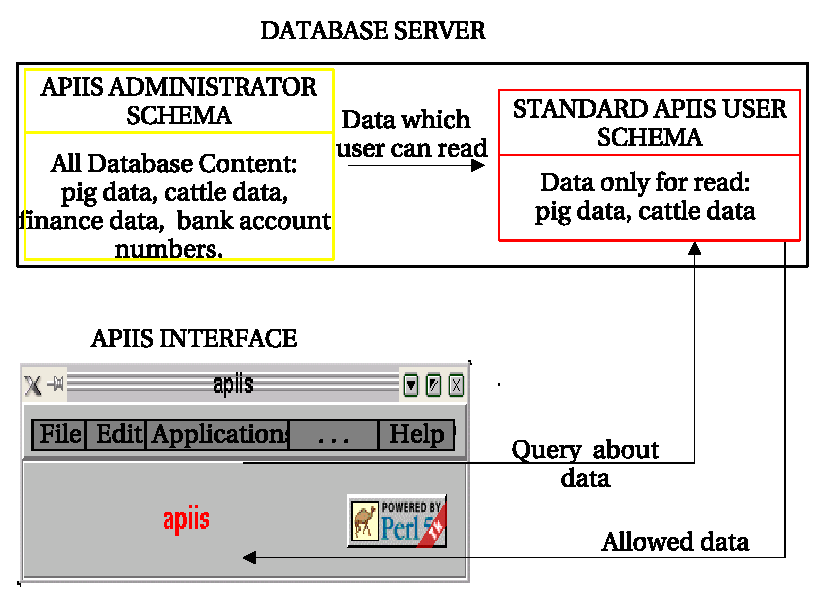
\includegraphics[scale=1]{./access-control/readingdata.eps}
   \caption{Reading data from the database}
   \label{fig:readingdata}
\end{center}
\end{figure}
\section{Remarks}
Implementation of the Security System is in the Perl Programming Language. 

